\documentclass{article}

\usepackage[margin=.75in]{geometry}
\usepackage{hyperref, graphicx, listings, multicol}
\graphicspath{ {./img/} }
\hypersetup{
  colorlinks=true
}

\title{Space Partitioning Algorithms and k-d Tree Construction}
\author{Ari Madian}

\begin{document}
\begin{center}
  \Large\textbf{Space Partitioning Algorithms and k-d Tree Construction}\\
  \textit{CSE 373 wi21 Research Project}\\
  Ari Madian
\end{center}

\tableofcontents
\pagebreak

\section{Motivation}
The thing that originally attracted me to this problem is the mention of swarm intelligence in the description.
I had previously tinkered with game development and controlling agents in the game with some really basic AI, so
swarm intelligence and the idea of the algorithms behind some game AIs, and the Intel drone swarms.

While working on the project, I was reminded of elements of algorithm analysis, recurrence relations, and sorting
algorithms. I was also reminded of a lot of what we studied regarding trees, balancing them, and searching them - particularly binary search trees.

\section{Explanation}
The three algorithms each take slightly different approaches to partitioning. Uniform partitioning is the least precise, but the fastest to build.
Quadtrees are in the middle of the road, offering slightly slower build times than uniform partitions, but faster search times since the tree is more balanced.
I say "balanced" even though uniform partitioning doesn't actually build a tree.

k-d trees are the slowest to build since the construction algorithm is much more intentional with picking \textit{where} to
partition, and as such, produce a much more balanced tree than quadtree partitioning. Since k-d trees produce more balanced
search trees, the search tends to be relatively fast since the search algorithm is able to eliminate partitions more efficiently.

I made an example 2d space on desmos to illustrate how partitioning will work with each method. This is the non-partitioned space:

\begin{center}
  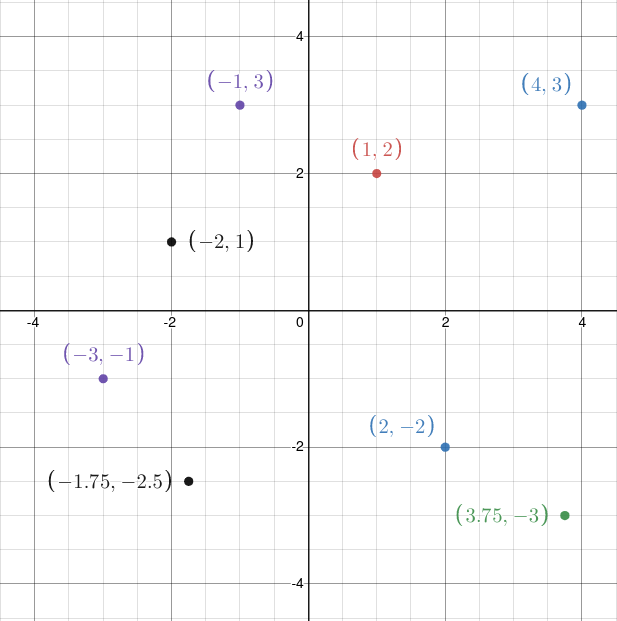
\includegraphics[width=.75\textwidth]{desmos-graph}
\end{center}

\subsection{Quadtrees}
Quadtrees generally are a tree structure in which each node has exactly four children. They can be used for space
partitioning by choosing to simply split each partition into four equally sized smaller partitions.

\begin{figure}[h]
  \centering
  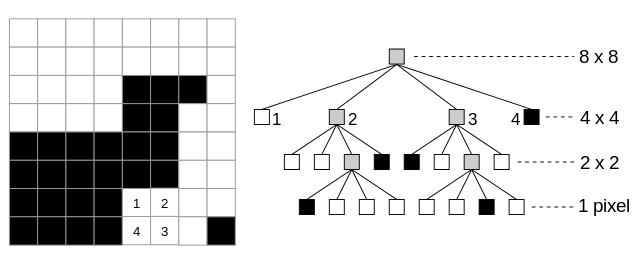
\includegraphics[width=0.75\textwidth]{quadtree.png}
  \caption{From the \href{https://en.wikipedia.org/wiki/Quadtree}{quadtree wikipedia page}.}
\end{figure}

Here you can see a representation of how an 8x8 bitmap would be partitioned into a quadtree structure.
The diagram is a bit confusing since it marks 1, 2, 3, and 4 as individual pixels on the bitmap, but gives those marks to 4x4 partitions on the tree.
The 1, 2, 3, and 4 markings are actually to say that the assignment of these numbers to their quadrants goes clockwise from the top left quadrant.

Here's an example of how quadtree partitioning would look:

\begin{center}
  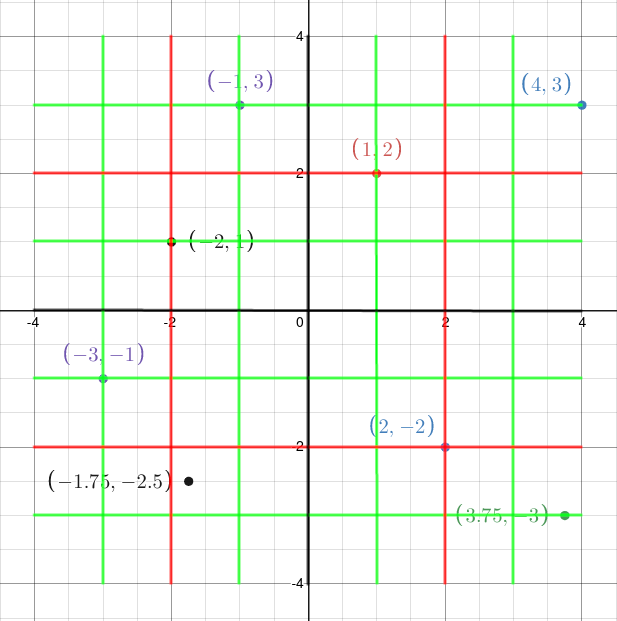
\includegraphics[width=.5\textwidth]{desmos-quad}
\end{center}

In terms of the image from Wikipedia above, the black lines represent the 8x8 node, the red lines represent the 4x4 node, and the green lines represent the 2x2 node.
Each white square separated by the lines represents a pixel, or more generally, an atomic partition of some space.

\subsection{k-d trees}
k-d trees are binary search trees where every leaf node represents a point on the graph, and other nodes represent partitions in the graph.

They differ from quadtrees because they use sorting or median finding algorithms to find a median point at which to partition the graph.
Because k-d trees take extra time in construction to try and ensure a more balanced tree, they generally offer better search runtimes.

An example of kd-tree space partitioning using my desmos chart looks like this:
\begin{multicols}{2}
  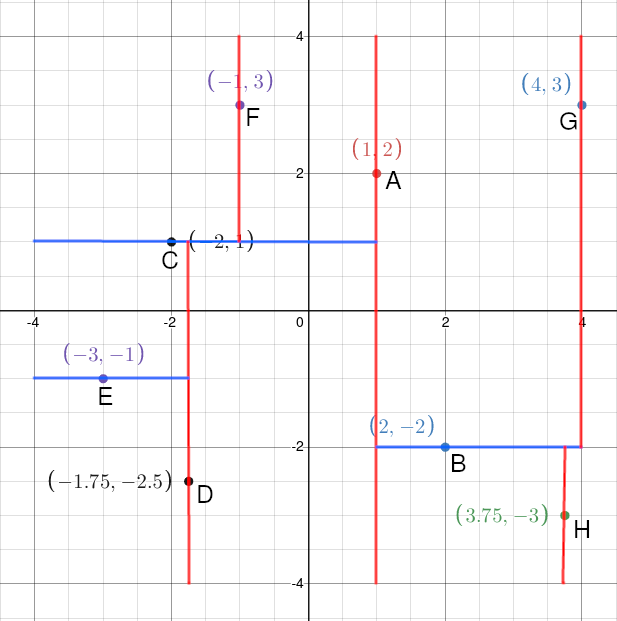
\includegraphics[width=.5\textwidth]{desmos-kd}
  \columnbreak
  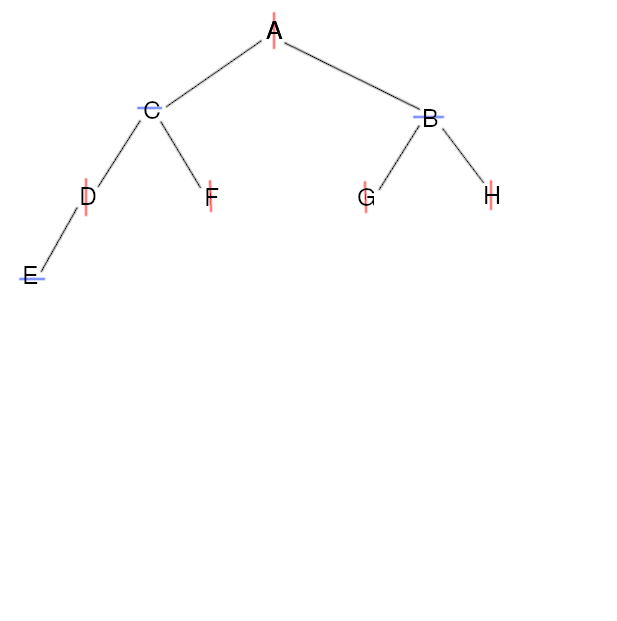
\includegraphics[width=.45\textwidth]{kd-tree}
\end{multicols}

The partitions were made in alphabetical order, sorted by x coordinate. Here's a table showing the partitioning process of the space above:

\subsubsection{k-d tree Construction}
The k-d tree construction algorithm has two main dominating factors: sorting the point list, and constructing the left and right subtrees.

Construction of the subtrees will always be approximately $\theta(log(n))$ time because similarly to binary search, we reduce the amount
of work we have to do by half at each successive level of depth in the tree.

Here is the pseudocode for k-d tree construction from the \href{https://en.wikipedia.org/wiki/K-d_tree}{k-d tree Wikipedia page}.
\begin{lstlisting}
  function kdtree (list of points pointList, int depth)
  {
    // Select axis based on depth so that axis cycles through all valid values
    var int axis := depth mod k;

    // Sort point list and choose median as pivot element
    select median by axis from pointList;

    // Create node and construct subtree
    node.location := median;
    node.leftChild := kdtree(points in pointList before median, depth+1);
    node.rightChild := kdtree(points in pointList after median, depth+1);
    return node;
  }
\end{lstlisting}

\begin{multicols}{2}
Here's a basic asymptotic analysis of this algorithm (assuming that merge sort is used):
\begin{tabular}{ c | c }
  Step & Runtime \\
  \hline
  Select Axis & $\theta(1)$ \\
  Sort Point List & $\theta(n log(n))$ \\
  Select Median Point & $\theta(1)$ \\
  Construct left Subtree & $\theta(log(n))$ \\
  Construct right Subtree & $\theta(log(n))$
\end{tabular}
\end{multicols}

\subsection{Uniform Partitioning}
Uniform partitioning is the simplest approach in terms of construction and implementation. All it really does is split some space into
uniform rectangular sections, also known as "buckets" or "bins".

The bins are represented as an array, and each item in the space is represented by a linked list node in its repective bin.

Here's an example using my desmos graph of how uniform partitioning on the space would look.

\begin{center}
  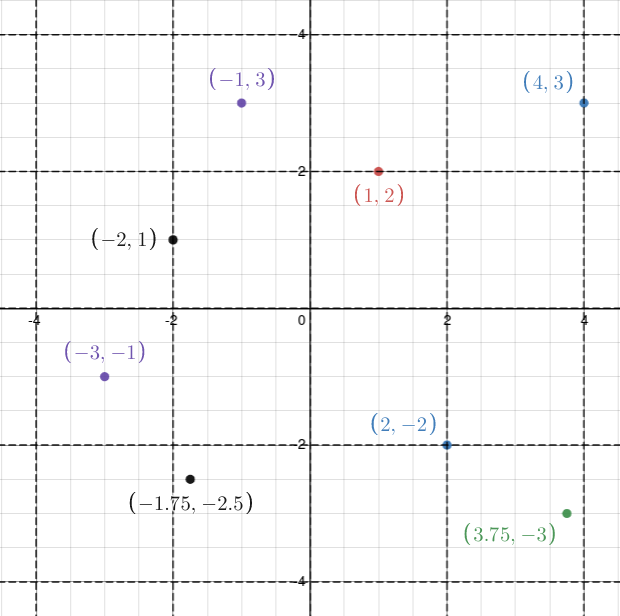
\includegraphics[width=0.5\textwidth]{desmos-uniform}
\end{center}

\section{Merge Sort Runtime Proof}
We know that the main factors in the k-d tree construction algorithm are sorting the point list and constructing the subtrees.
Since we have two main parts, we can say that our total runtime for k-d tree construction is:

$$\theta([something] + [something])$$

For each call of the kdtree method, the asymptotic variable is the size of the point list, $n$.
Since we know that merge sort always results in a $\theta(n log(n))$ runtime, we can say that the runtime of the first dominating
part of k-d tree construction gives a $\theta(n log(n))$ runtime, giving us a total runtime of

$$\theta((n log(n)) + [something])$$

Then, since we know that construction of each subtree has an asymptotic runtime of $log(n)$, we can then say that our total runtime is

$$\theta((n log(n)) + (log(n)))$$

However, since we are sorting the point list for each run, we actually have to say that our total runtime is

$$\theta((n log(n)) * (log(n))) = \theta(n * log(n) * log(n)) = \theta(n*log^{2}(n)),\ or\ \theta(n log^{2}(n)).$$

\section{Alternative Construction Method}
Since the $n log(n)$ merge sort dominates the $log(n)$ subtree construction, we may want to look for a more
efficient method of selecting a partition, while still maintaining a relatively balanced tree.

Since the asymptotic variable of merge sort is the number of items to be sorted, $n$, we probably want to look at
ways to reduce $n$. To do this, we could select a proportionally small subset of all $n$ points, then sort and pick the median of those.

Say we use my desmos graph. The x coordinates are [-1, 4, 1, -2, -3, 2, -1.75, 3.75], let's call it $l$.
In this case $n$ would be 8. We can reduce the runtime by half by randomly picking a subset of $l$, and sorting that, maybe [-3, -1.75, 3, 4].
Now we've reduced $n$ by half, and even though the correct median isn't in the subset, with a large enough data set, our
median from the subset may be close enough to the real median that we can still get a relatively balanced k-d tree.

Another possible approach is that since the first few partitions are the most important in getting a balanced tree, we could use
the subset strategy on depths of 3+.

This subset approach also allows us to fine tune our preference between precision and speed.
\end{document}
